\documentclass[11pt]{report}

\usepackage{epsf,amsmath,amsfonts}
\usepackage{graphicx}
\usepackage{color}
\usepackage{natbib}

\setlength{\textwidth}{6.5in}
\setlength{\oddsidemargin}{0in}
\setlength{\evensidemargin}{0in}
\setlength{\textheight}{8.5in}
\setlength{\topmargin}{0in}

\begin{document}

\title{
Sub-Ice Shelf Ocean Test
}
\author{MPAS Development Team}

\maketitle
\tableofcontents

%-----------------------------------------------------------------------

\chapter{Summary}

Here we propose a set of tests to answer the following questions:
\begin{enumerate}
\item How thin can MPAs-Ocean layers be compressed below land ice?
\item How steep can the edge of the floating ice shelf be?
\end{enumerate}
The domains are designed to be the simplest possible configurations to test the vertical coordinate, but realistic enough that it provides guidance for global simulations using full bathymetry, forcing, and realistic ice shelves.    The land ice will be imposed with a surface pressure, and MPAS-Ocean will run in 'z-star' mode, where layers contract in proportion to the displaced surface, like an upside-down sigma coordinate.  We hope to demonstrate the extent to which 'z-star' may be used under ice shelves.  the next step would be to make upper cells inactive if z-star does not work.  This is similar to z-level bathymetry but at the top, and is what Xylar implemented in POP.  Likely problems with the z-star formulations for large depressions and slopes are: numerical instabilities in thin layers; tight timestep constraints due to vertical CFL; and velocity errors due to steeply tilted layers.

%-----------------------------------------------------------------------

\chapter{Test Set-up}

The test domain is designed to mimic the geometry of the Pine Island Glacier (PIG), which has a steeply sloped ice shelf bottom of 500 m over 30 km (Figure \ref{figure:pig observations}, \citet{Jenkins_ea10ngeo}).  Parameters are listed in Table \ref{table:ideal test parameters}.  The ocean will be run in stand-alone mode, without a land ice model or coupler.  There will be no fluxes from the ice shelf, and the ocean will be depressed but a surface pressure due to the weight of the ice shelf.  The domain is 50 km wide with a constant Coriolis parameter of $-1.4\times10^{-4}$ s$^{-1}$, which is appropriate for the PIG latitude of 75$^o$ S.  Simulations will be performed with both periodic and solid  boundaries in the $x$ direction.

The ocean will consist of 22 layers that compress proportionally below the ice sheet, so that they are each 50 m thick in the open ocean and 4.5 m thick at the cavity (Figure \ref{figure:ice shelf domain}a).  The cavity thickness, $A$, will be varied from 100m to 1m to test how thin the layers may function properly.  The cavity thickness will be decreased by increasing the surface pressure so that the whole ice sheet is uniformly deeper.  The upper slope at the end of the ice shelf will be controlled by varying $B$ from 0 to 30 km, to test the model's ability to include steep slopes.

Three tests will be conducted that are each progressively more complex (Figure \ref{figure:ice shelf domain}).
\begin{enumerate}
\item {\bf Quiescent cavity:} Stratification in the vertical only and no wind stress should produce zero ocean velocity.  Nonzero velocities are model errors, most likely due to steeply tilted layers when using the nonlinear equation of state.
\item {\bf Driven cavity:} The addition of wind forcing and a horizontal salinity gradient will drive a circulation up the ice shelf bottom.  There is no analytic solution here, so success is judged by model stability.
\item {\bf Bottom Topography:} In addition to the flat-bottom case, bathymetry may be added to show the combination of z-level land cells with compressed z-star layers.
\end{enumerate}

Tests will be conducted with both a linear equation of state and the nonlinear equation of state by \citet{Jackett_McDougall95jaot}.  The momentum equation includes the $\nabla z^{mid}_{k}$ term, which is the pressure gradient correction due to tilted coordinate surfaces, computed as in \citet[Section 2, method 4]{Shchepetkin_McWilliams03jgr}.  Weighted averaging of the density and vertical coordinate \citep[Section 3]{Song98mwr,Shchepetkin_McWilliams03jgr} is not included.  Velocity errors in tilted coordinates due to the compressibility of sea water \citep[Section 7]{Shchepetkin_McWilliams03jgr} should occur when testing with a nonlinear equation of state.

Additional settings are similar to those used in real-world configurations described in \citet{Ringler_ea13om}.  This includes a quadratic bottom drag with a coefficient of 0.01 and monotonic flux-corrected tracer transport \citep{Skamarock_Gassmann11jcp}, with third order reconstruction of the tracer values at the cell edges.  The horizontal turbulence closure is a simple hyperviscosity ($-\nabla^4$) operator with coefficients of $\nu_h = \nu_0 (\Delta x / \Delta x_0)^3$ with $\nu_0=5\times10^{10}$ and $\Delta x_0=15$ km grid cells.  Zero horizontal diffusion is applied to the tracers.  The vertical mixing is Richardson number-based, with background viscosity and diffusion of $10^{-4}$ and $10^{-5}$ m$^2$ s$^{-1}$, respectively.

\begin{figure}[tbh]
\center
\includegraphics[width=3in]{f/Jenkins_ea10ngeo_fig4b.pdf}
\caption{Observations below the Pine Island Glacier, from \citet{Jenkins_ea10ngeo}.  Ocean salinity and slope of the ice shelf were considered in designing the test domain.}
\label{figure:pig observations}
\end{figure}

\begin{figure}[tbh]
\center
(a)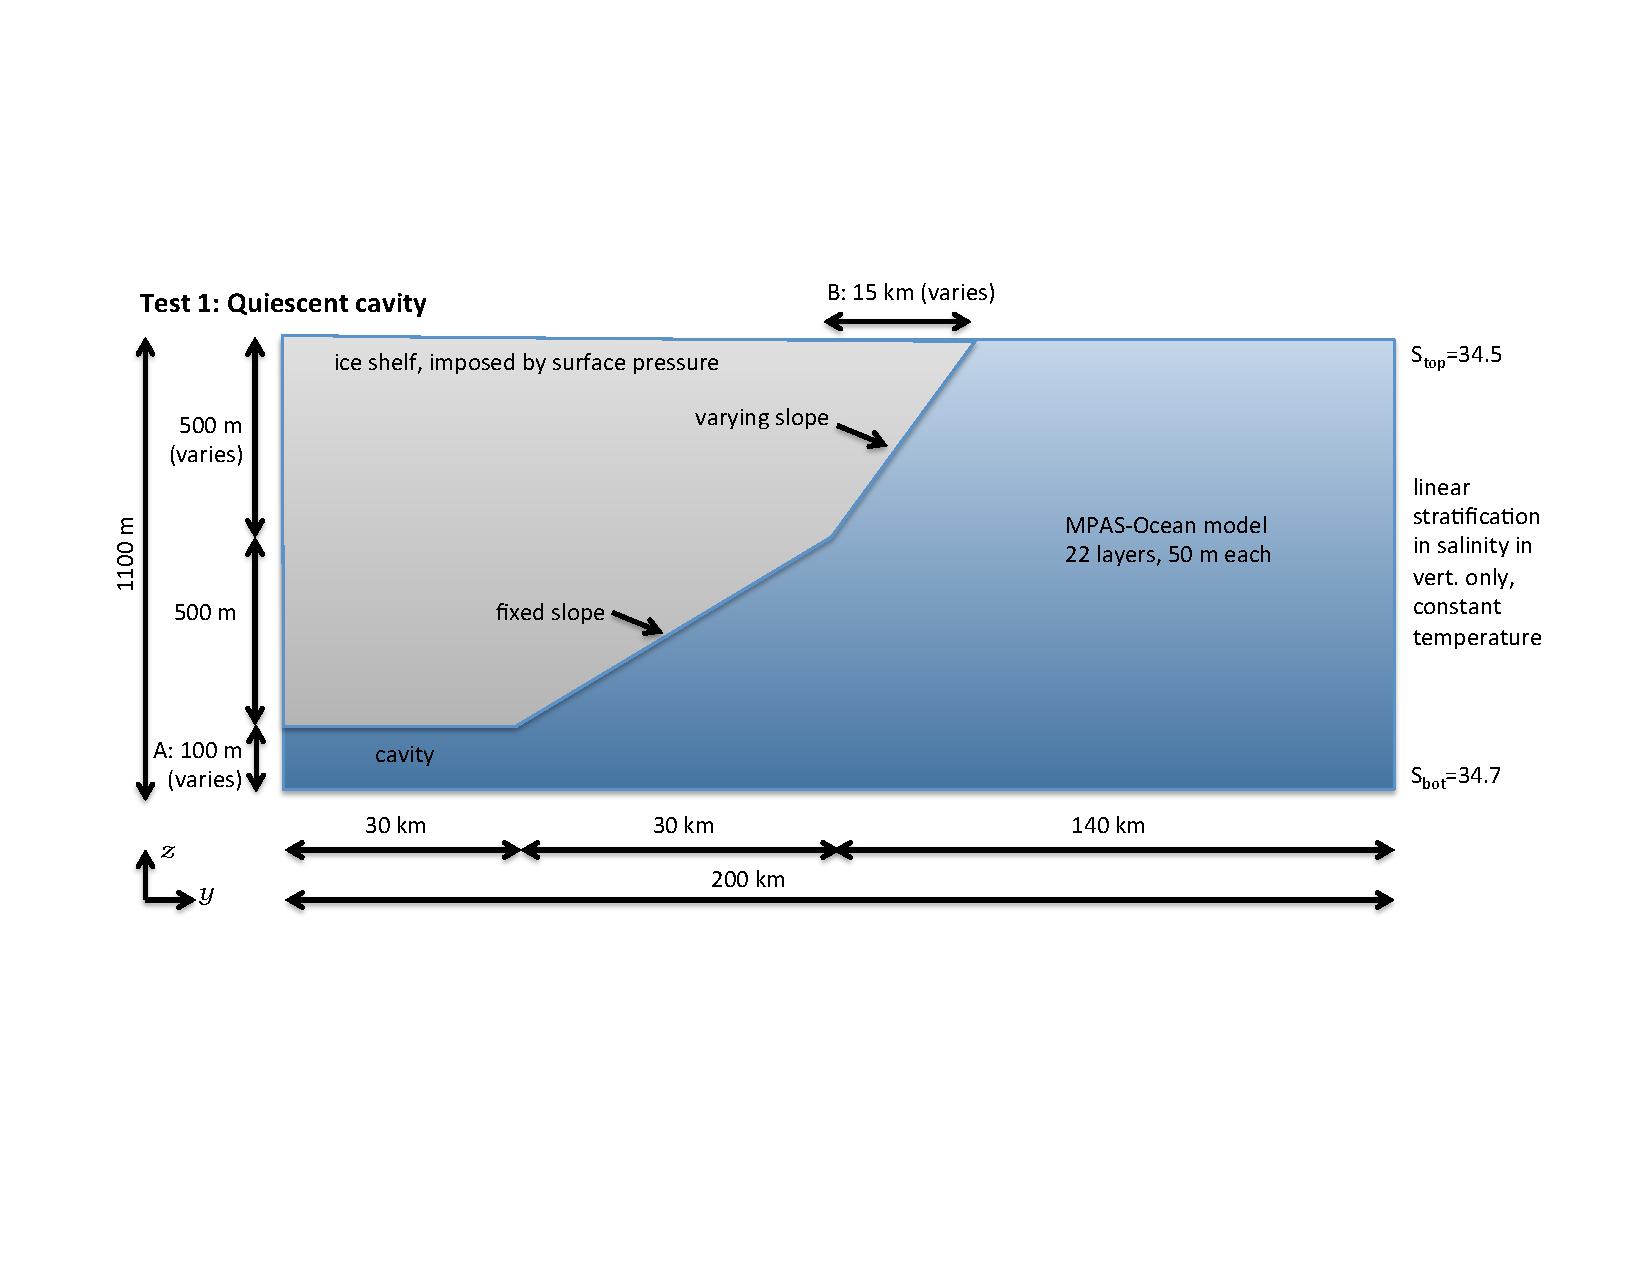
\includegraphics[width=5.75in]{f/sub-ice_shelf_test1.pdf}\\
\vspace{.2in}
(b)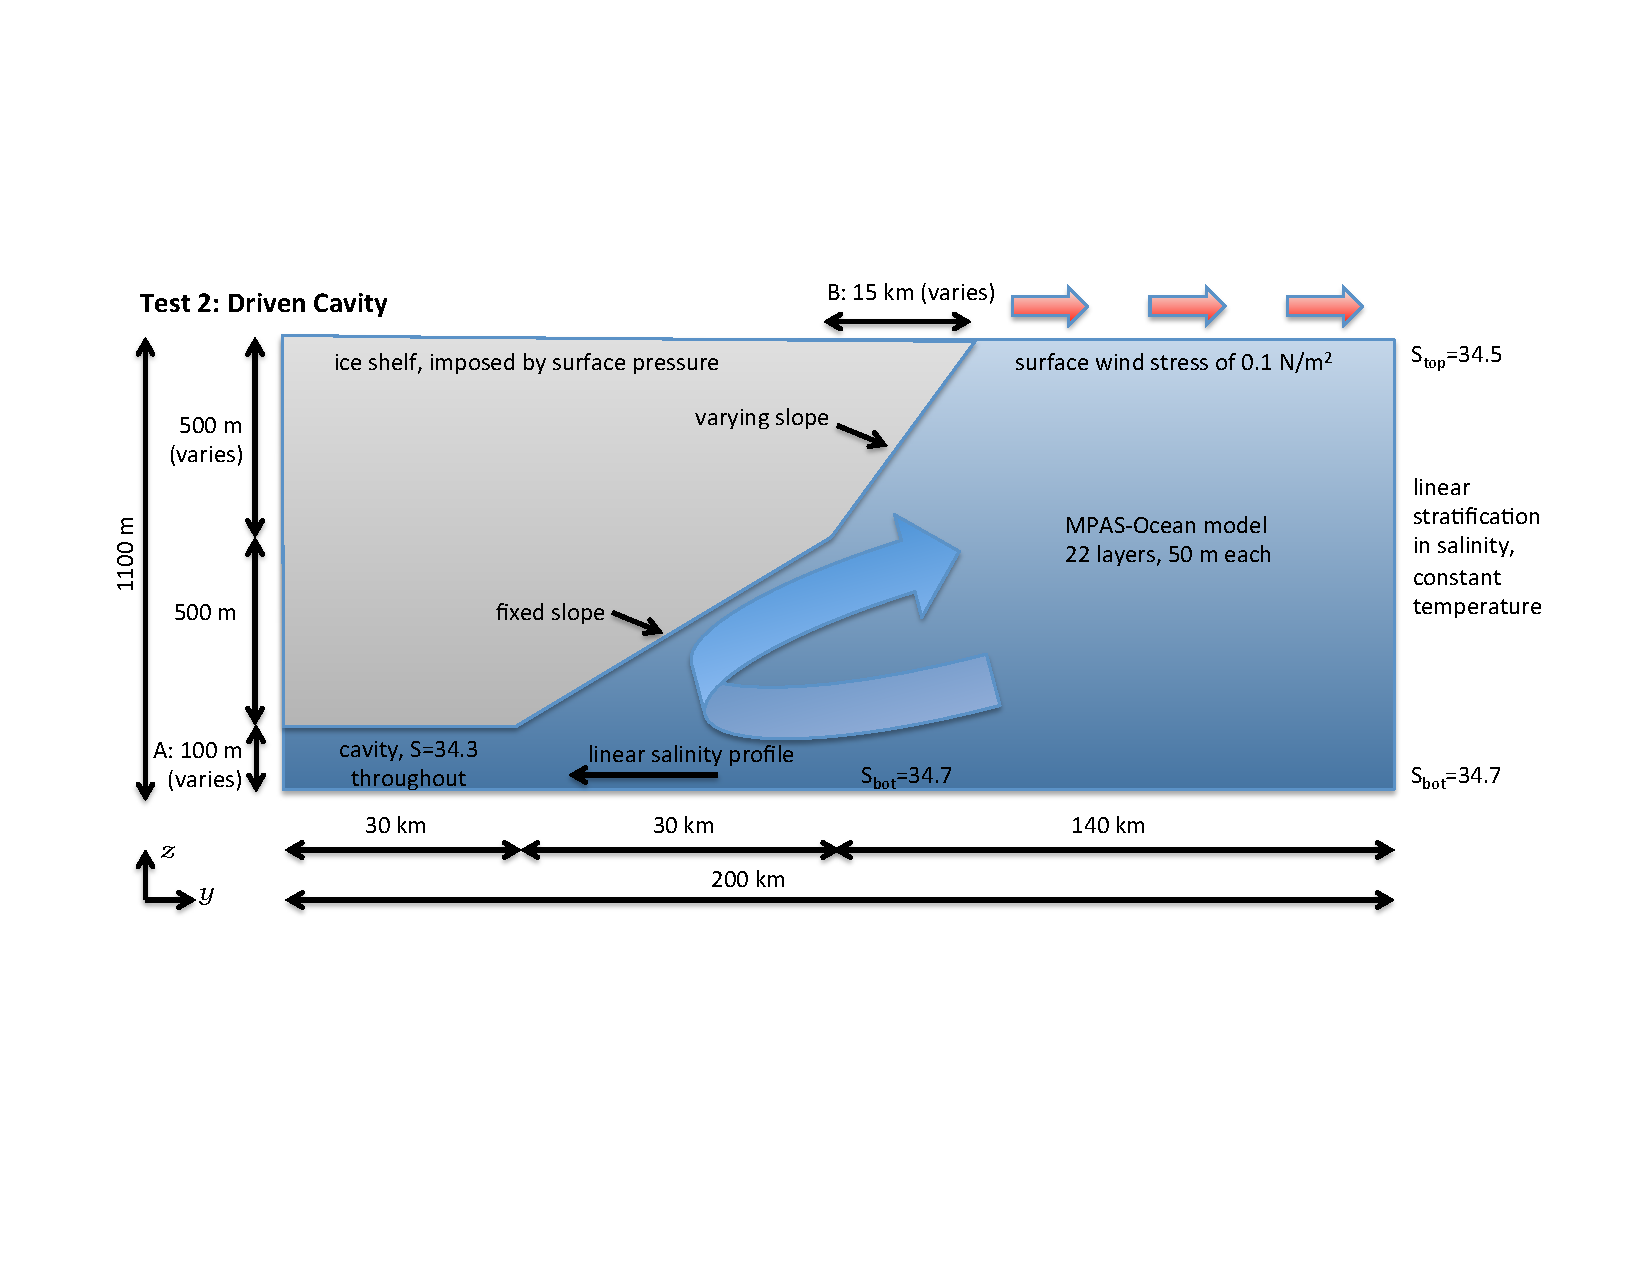
\includegraphics[width=5.75in]{f/sub-ice_shelf_test2.pdf}\\
\vspace{.2in}
(c)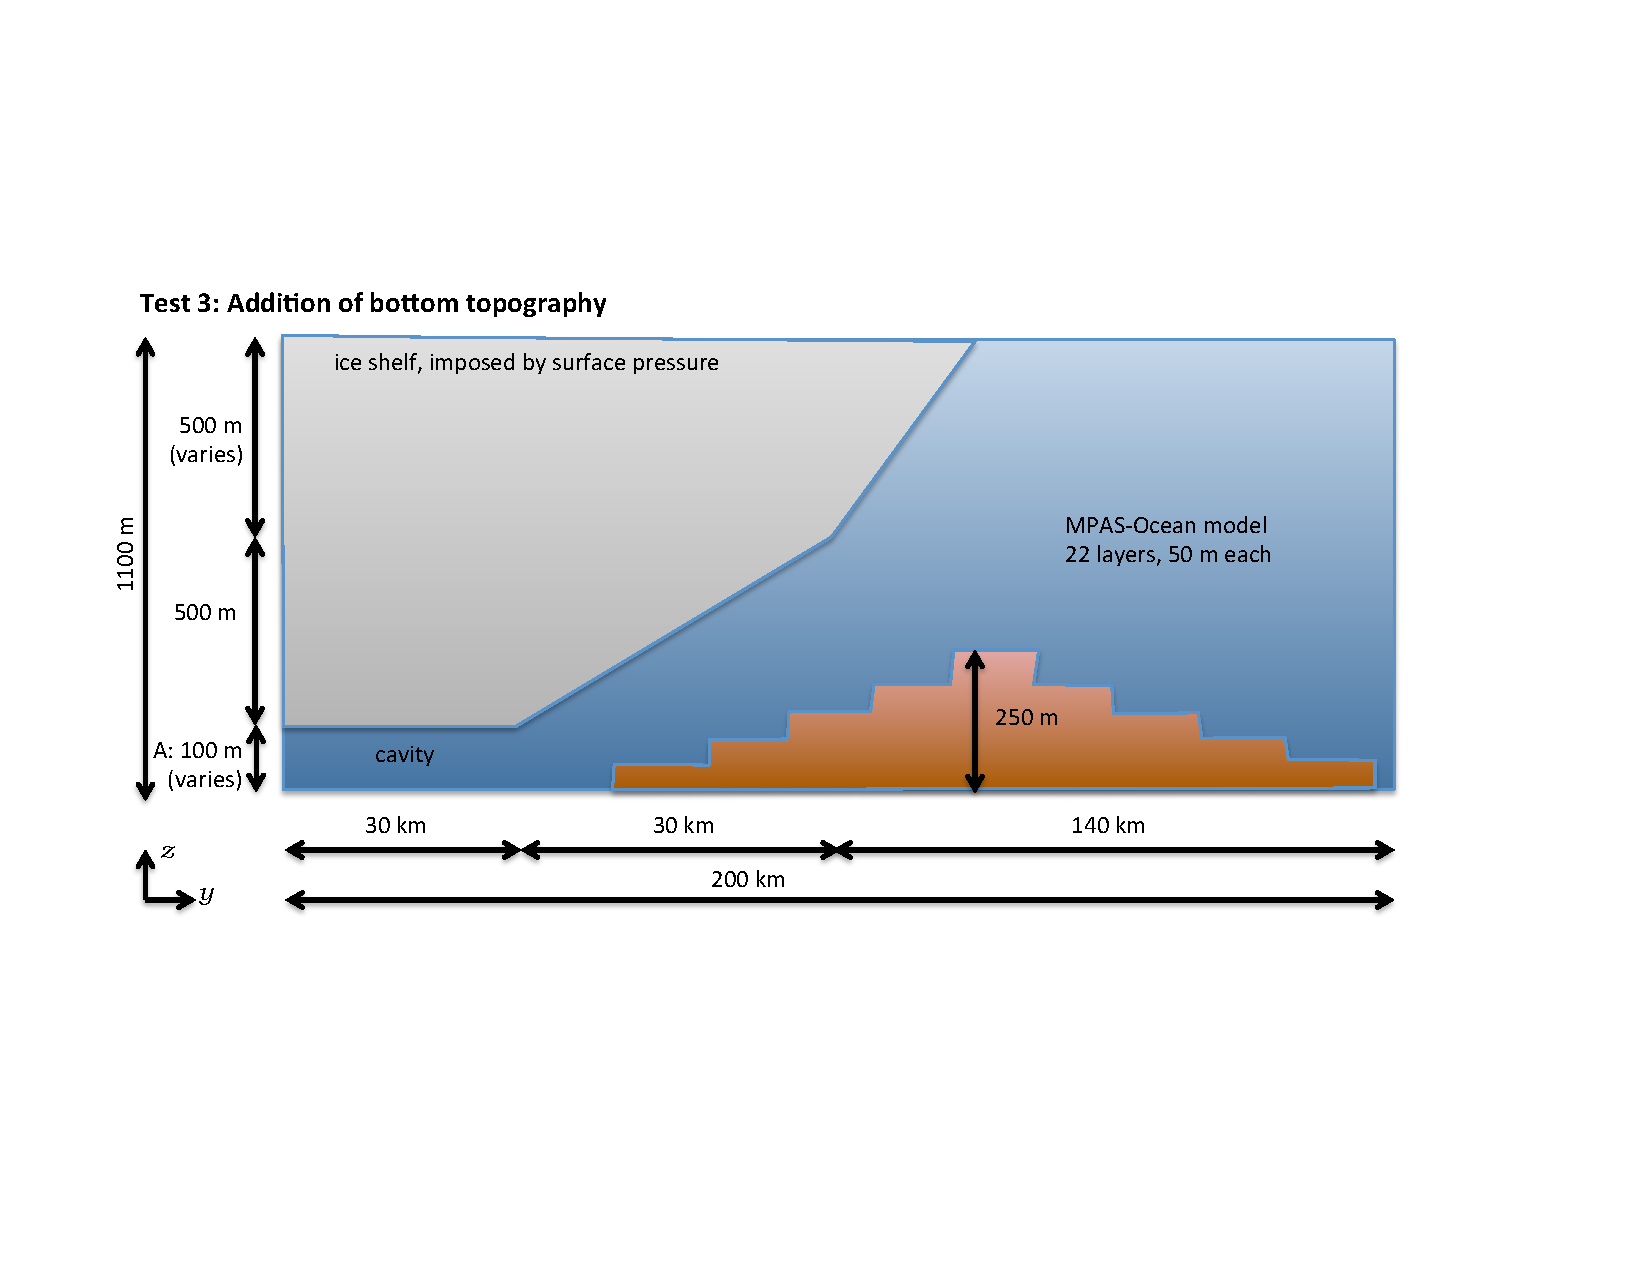
\includegraphics[width=5.75in]{f/sub-ice_shelf_test3.pdf}\\
\caption{Domain of the ice shelf test cases.  The cavity thickness (A) and width of ice shelf edge (B) are the parameters that will be varied.}
\label{figure:ice shelf domain}
\end{figure}


\begin{table}[tbh] 
\caption{Parameter settings for sub-ice shelf test cases.}
\vspace{0.5cm} \centering 
\begin{tabular}{r|c } 
\hline\hline & case 1 \\
\hline 
domain size $x$ &  50 km\\
domain size $y$ & 200 km\\
domain size $z$ &  1100 m \\
number layers& 22 \\
layer thickness & 50 m in open ocean \\
grid cell size, km  & 15, 5, 1 \\
time step $\Delta t$, s & 600, 200, 40 \\
$\nabla^4$ $\nu_h$, m$^2/$s & 5e10, 1.8e9, 1.5e7 \\
$\nu_v$, m$^2/$s & rich, bkrd of $1\times10^{-4}$ \\
$\kappa_h$, m$^2/$s & 0 \\
$\kappa_v$, m$^2/$s & rich, bkrd of $1\times10^{-5}$ \\
bottom drag & 0.01 \\
Coriolis, s$^{-1}$ & $-1.4\times10^{-4}$ s$^{-1}$ \\
temperature & 1 C throughout \\
equation of state & linear and Jackett-McDougall \\
run duration& 24 hours \\
\hline 
\end{tabular} \label{table:ideal test parameters}
\end{table}

%-----------------------------------------------------------------------

\bibliographystyle{elsarticle-harv}
\bibliography{sub-ice_shelf_ocean_test}

%-----------------------------------------------------------------------

\end{document}
